% Exam Template for UMTYMP and Math Department courses
%
% Using Philip Hirschhorn's exam.cls: http://www-math.mit.edu/~psh/#ExamCls
%
% run pdflatex on a finished exam at least three times to do the grading table on front page.
%
%%%%%%%%%%%%%%%%%%%%%%%%%%%%%%%%%%%%%%%%%%%%%%%%%%%%%%%%%%%%%%%%%%%%%%%%%%%%%%%%%%%%%%%%%%%%%%

% These lines can probably stay unchanged, although you can remove the last
% two packages if you're not making pictures with tikz.
\documentclass[11pt]{exam}
\RequirePackage{amssymb, amsfonts, amsmath, latexsym, verbatim, xspace, setspace, graphicx, listings}
\RequirePackage{tikz, pgflibraryplotmarks}

% By default LaTeX uses large margins.  This doesn't work well on exams; problems
% end up in the "middle" of the page, reducing the amount of space for students
% to work on them.
\usepackage[margin=1in]{geometry}
\usepackage{graphicx}
\usepackage{listings}

% Here's where you edit the Class, Exam, Date, etc.
\newcommand{\class}{Intermediate Exp. Physics II}
\newcommand{\prof}{Prof. Andrew Kent}
\newcommand{\term}{Spring 2016}
\newcommand{\examnum}{Midterm}
\newcommand{\examdate}{March 21, 2016}
\newcommand{\timelimit}{Due in class before lecture Monday, March 28, 2016}

% For an exam, single spacing is most appropriate
\singlespacing
% \onehalfspacing
% \doublespacing

% For an exam, we generally want to turn off paragraph indentation
\parindent 0ex

\begin{document}

% These commands set up the running header on the top of the exam pages
\pagestyle{head}
\firstpageheader{}{}{}
\runningheader{\class}{\examnum\ - Page \thepage\ of \numpages}{\examdate}
\runningheadrule

\begin{flushright}
\begin{tabular}{p{2.8in} r l}
\textbf{\class} & \textbf{Name (Print): Caspar Lant} & \makebox[2in]{\hrulefill}\\
\textbf{\prof} \\
 \textbf{Lab Instructor: David Mykytyn} \\
\textbf{\term}: \textbf{\examnum} &&\\
\textbf{\examdate} &&\\
\end{tabular}\\
\end{flushright}
\textbf{Time Limit: \timelimit} % {\hrulefill}

\rule[1ex]{\textwidth}{.1pt}

This exam has \numquestions\ problems.  Enter you name on the top of this page, and put your initials
on the top of every page you submit, in case the pages become separated. You may include
additional sheets of paper in your answers to this exam (i.e. not all your answers are expected
to be on these exam sheets.)\\

This is open book (open everything) take home exam. You are expected to work independently on the exam--not discuss it
with others in or outside the class. It is due in class before the lecture on Monday, March
28, 2015. Please write your answers out completely.\\

Attempt to answer all the problems and show your work, as this is required to get full credit for your answers and will be used to determine partial credit. Good luck!
\\

\newpage % End of cover page


\hfill
\begin{minipage}[t]{2.3in}

\vspace{0pt}
%\cellwidth{3em}
\gradetablestretch{2}
\vqword{Problem}
\addpoints % required here by exam.cls, even though questions haven't started yet.
\gradetable[v]%[pages]  % Use [pages] to have grading table by page instead of question

\end{minipage}

\newpage

%%%%%%%%%%%%%%%%%%%%%%%%%%%%%%%%%%%%%%%%%%%%%%%%%%%%%%%%%%%%%%%%%%%%%%%%%%%%%%%%%%%%%
%
% See http://www-math.mit.edu/~psh/#ExamCls for full documentation, but the questions
% below give an idea of how to write questions [with parts] and have the points
% tracked automatically on the cover page.
%
%
%%%%%%%%%%%%%%%%%%%%%%%%%%%%%%%%%%%%%%%%%%%%%%%%%%%%%%%%%%%%%%%%%%%%%%%%%%%%%%%%%%%%%
\setstretch{1.5}
\begin{questions}
\question {\bf Spin Resonance.}
\begin{parts}
\part
The directional derivative of $\vec S$ in the the $\hat S$ direction is equivalent to the rate of change of the magnitude of $\vec S$. Expressed mathematically, $\frac{\rm d}{{\rm d}t} = $
We know that $\vec S$ and $\vec \mu$ point in the same direction, because $\vec{\mu}=g_s \mu_B\vec{S}/\hbar$. We know that for the case
${\rm A {\bf \hat i} = B{\bf \hat i} \times C{\bf \hat j}}$, A or B or C must be zero. Taking the nontrivial case where $\vec \mu$ and $\vec B$ are nonzero, we see that $\frac{\rm d}{{\rm d} t} = 0$. This means that the magnitude of $\vec S$ must be time-independent.
\[\frac{\rm d}{{\rm d} t} \vec S = \vec\tau = \vec\mu\times\vec B\]

\part
If we assume an orthonormal coordinate system, and at at $t=0, \vec S = S\hat x$, and $\vec B = B_0 \hat z$, we know that $\vec\mu$ points in the $y$-direction, because of the orthogonal nature of the cross product. Assuming that our dipole precesses, we are free to say that at a later time $t$, $\vec S$ will point in the direction given by $R_{\theta} \cdot S \hat x $, where $R_{\theta}$ is the rotation matrix, and $\theta$ is given by $\omega t$... We know that $\vec \tau = \frac{\rm d}{{\rm d} t}\vec S \sin\phi = S \frac{{\rm d} \theta}{{\rm d}t}$
because $\frac{\rm d}{{\rm d} t}|\vec S| = 0$. $\phi$ is also zero in this case, because $\vec S$ points along the $x$-axis.
$\tau = |\mu||B|\sin\phi = \mu_B B_0 = \dfrac{g_s \mu_B}{\hbar}|S| B_0 = \frac{{\rm d} \theta}{{\rm d}t}|S| =\omega |S| $
Dividing the above equation by $|S|$, we obtain: \[\omega = \dfrac{g_s \mu_B}{\hbar} B_0\]
\part
\[30{\rm MHz} = \dfrac{g_s \mu_B}{\hbar} (1{\rm mT}) \Rightarrow \frac{30{\rm MHz}}{1{\rm mT}}\hbar = g_s\mu_B = 3.163 \times 10^{-24} \ {\rm m^2 A}\]
\medskip
\part If the orientation of the dipoles is orthogonal, they will not interact with eachother.

\end{parts}

\newpage
\question {\bf Blackbody radiation.}
\begin{parts}
\part
Thanks to Planck, we know that the energy of a photon is directly proportional to its frequency by a factor of Planck's constant. If we take a Boltzmann distribution of possible energy states, we would expect there to be relativly few high energy photons radiated from our blackbody, compared to the average energy of the body. Because the energy at a given frequency is quantized by photons, there is some minimum threshold for each energetic mode of the blackbody. This resolves the so-called ``Ultraviolet Catasrophe".

\part
\begin{figure}[h]
    \centering
    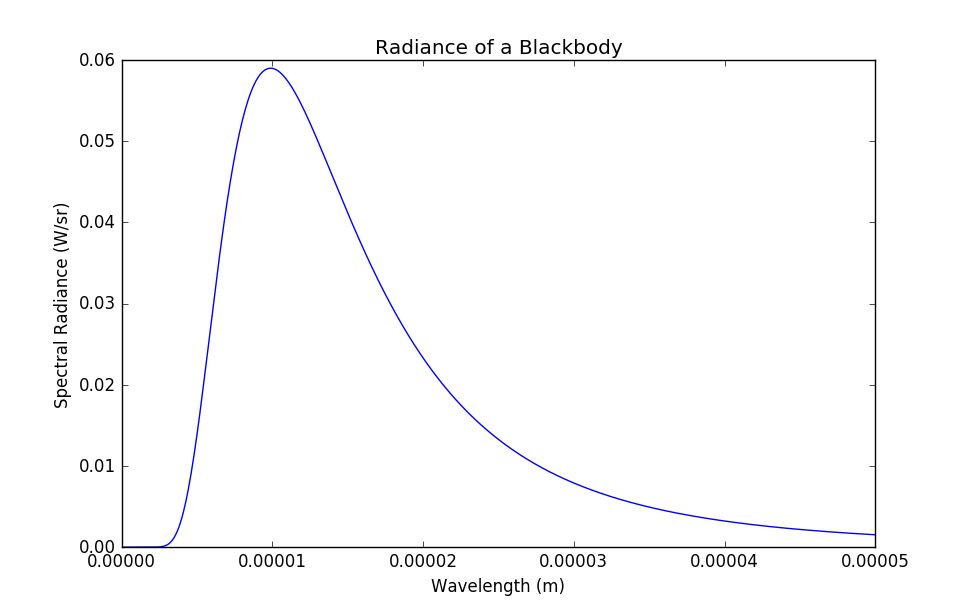
\includegraphics[width=0.8\textwidth]{blackbody.png}
    \caption{Blackbody Radiation at Room Temperature}
\end{figure}
\setstretch{0.5}
\lstinputlisting[language=Python]{blackbody.py}
\setstretch{1.5}

\end{parts}

\question {\bf Photoelectric Effect.}
\begin{parts}
\part
Fermi electrons in a metallic lattice that absorb a photon with energy below the minimum release threshold are briefly energized, and quickly fall back into their resting state, emitting a photon of equivalent energy in the process. This is an explanation as to why metals are so lusterous.
You may ask: ``What if two photons hit a fermi electron at the same time? Wouldn't the energy be sufficient to release the electron? Why don't we see this happen more often?''
We can imagine that electrons are only struck by one photon at a time because the duration of the energy transfer described above is nearly instantaneous.

\part
\begin{figure}[h]
    \centering
    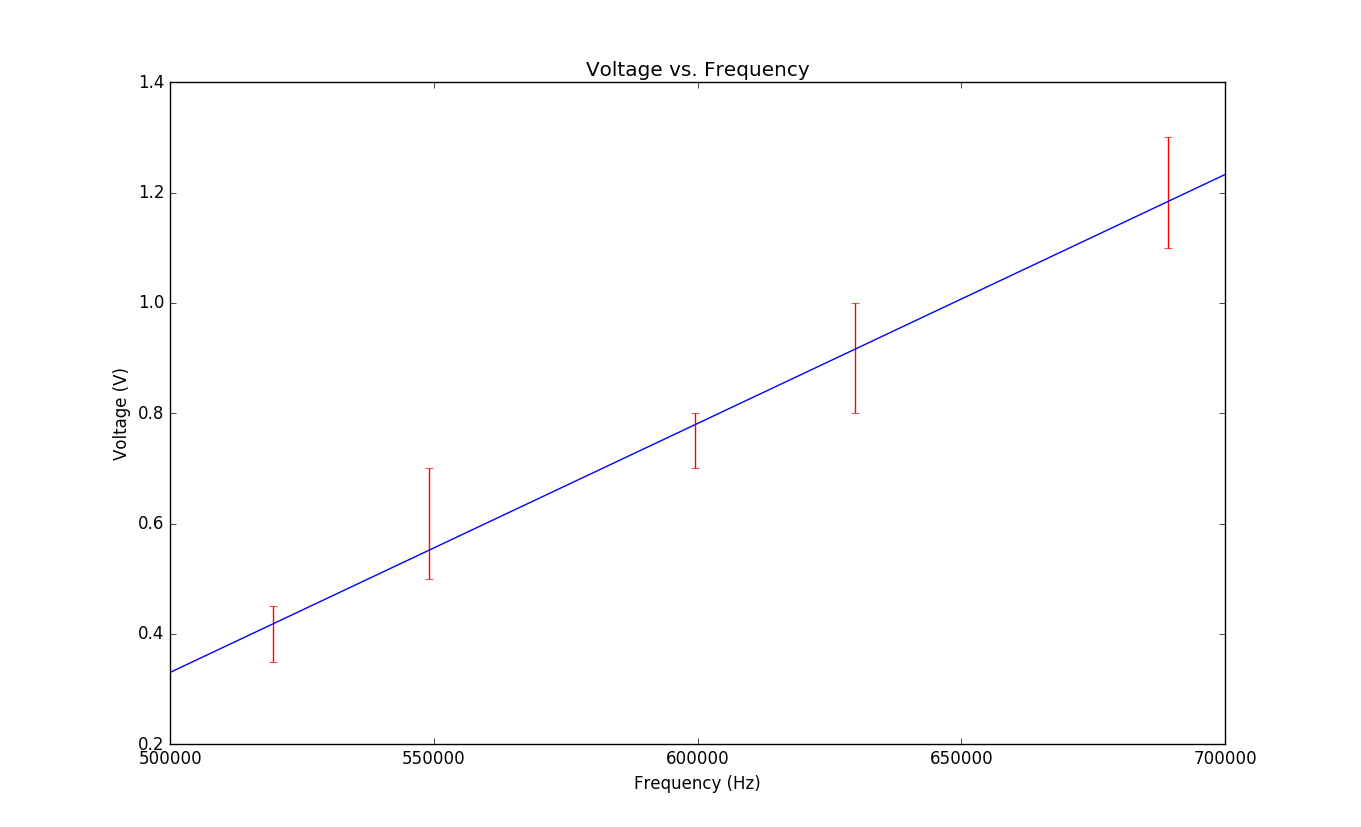
\includegraphics[width=0.8\textwidth]{plot.png}
    \caption{Plot With Uncertainties and Line Fit}
\end{figure}
\setstretch{0.8}
\lstinputlisting[language=Python]{planck.py}
\setstretch{1.5}

\part
My experimental value for Planck's constant was $7.2794 \times 10^{-34} \ {\rm m^2 \cdot kg}/{\rm s} \ \pm\ 9.0437 \times 10^{-35} $
My experimental value for the work function was $1.9233 \times 10^{-19} {\rm\ eV} \ \pm\ 5.2386 \times 10^{-20} $

\end{parts}
\newpage

\question {\bf Propagation of Uncertainties.}
Suppose we measure $N$ pairs of experimental values $(x_i, y_i)$ of two variables $x$ and $y$ that are predicted to satisfy a linear relation $y = mx + b$. Further, suppose the $x_i$ have negligible uncertainty and the $y_i$ have different uncertainties $\sigma_i$. (That is $y_1$ has uncertainty $\sigma_1$, and so on.) We can define the weight of the $i$th measurement as $w_i = 1/\sigma_i^2$.

\begin{parts}
\part From Taylor's book, we see that the unweighted estimates of $b$ and $m$ are:
\[b_{\rm unweighted} = \dfrac{\Sigma x^2 \Sigma y - \Sigma x \Sigma xy}{N\Sigma x^2 - \left(\Sigma x\right)^2}
\qquad\text{and}\qquad
m_{\rm unweighted} = \dfrac{N\Sigma xy -\Sigma x \Sigma y}{N\Sigma x^2 - \left(\Sigma x\right)^2}\]

Because the uncertainty in $y$ is different for each value of $y$, it must be included in the sum. We can achieve this quite easily:
\[b_{\rm weighted} = \dfrac{\Sigma \omega x^2 \Sigma \omega y - \Sigma \omega x \Sigma \omega xy}
{\Sigma \omega \Sigma \omega x^2 - \left(\Sigma \omega x\right)^2}
\qquad\text{and}\qquad
m_{\rm weighted} = \dfrac{\Sigma \omega \Sigma\omega xy -\Sigma \omega x \Sigma \omega y}
{\Sigma \omega \Sigma \omega x^2 - \left(\Sigma \omega x\right)^2}\]

if the estimated uncertainties are constant of all values of $y$, $\Sigma\omega = N$, which is why $N$'s crop up in our unweighted estimates and dissapear in our weighted ones, as well as why we see an extra $\Sigma\omega$ term in the denominator in each equation (in leu of an `N').

\part
In the next page of Taylor's book, we see:
\[\sigma_b = \sigma_y \sqrt{\dfrac{\Sigma x^2}{N\Sigma x^2 - \left(\Sigma x\right)^2}}
\qquad\text{and}\qquad
\sigma_m = \sigma_y \sqrt{\dfrac{N}{N\Sigma x^2 - \left(\Sigma x\right)^2}}\]
Where $\Delta = N\Sigma x^2 - \left(\Sigma x\right)^2$. This again neglects the fact that uncertainty values $\sigma_y$ are not uniform across $y$, and must therefore be places within our sums:
\[\sigma_b = \sqrt{\dfrac{\Sigma\omega x^2}{\Sigma \omega \Sigma \omega x^2 - \left(\Sigma \omega x\right)^2}}
\qquad\text{and}\qquad
\sigma_m = \sqrt{\dfrac{\Sigma \omega}{\Sigma \omega \Sigma \omega x^2 - \left(\Sigma \omega x\right)^2}}\]
Again, $N$ becomes $\Sigma\omega$ because the values are weighted
\end{parts}

\end{questions}
\end{document}
